\JWlone{Design}

How did I solve the problem?

% #  INSPECTED HARDWARE  #######################################################
\JWltwo{Inspected Hardware}
\label{sec:hw}


% -  PRODUCTS  -----------------------------------------------------------------
\JWlthree{Products}
\label{sec:hw-products}

\begin{itemize}

\item Intel Core i7, 2600K, Sandy Bridge

\item ASUS foo bar

\end{itemize}


% -  SANDY BRIDGE CHARACTERISTICS  ---------------------------------------------
\JWlthree{Sandy Bridge's Characteristics}
\label{sec:sandy-bridge}

In this section, characteristics of the Sandy Bridge architecture are described
in detail.

\begin{figure}
  \centering
    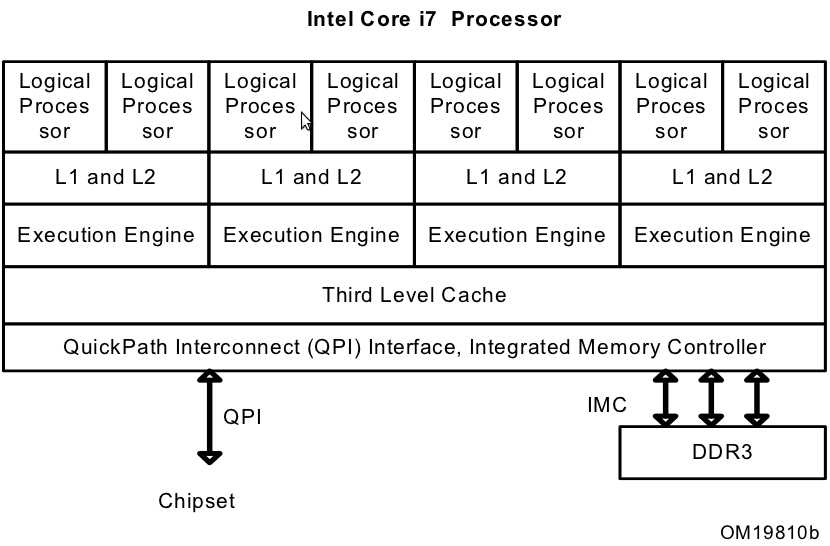
\includegraphics[width=\textwidth]{fig/intel-cache-orga.png}
  \caption{\JWPcpu cache organization (taken from \cite{intel2011softdev})}
  \label{fig:cache-orga}
\end{figure}


\JWlfour{General}

\begin{itemize}

\item organization: see \ref{fig:cache-orga}

\item L1 cache of \SI{64}{\kilo\byte} per core\cite{intel2011softdev}

\item L2 cache of \SI{256}{\kilo\byte} per core\cite{intel2011softdev}

\item shared L3 cache of \SI{8}{\mega\byte}\cite{intel2011softdev}

\end{itemize}


\JWlfour{PMU}
\label{sec:sandy-bridge-pmu}

\begin{itemize}

\item ca. 184 events available

\item 8 general-purpose performance counter registers available per core (4 in
      HT mode)

\item 3 fixed performance counter registers (CPU\_CLK\_UNHALTED, INST\_RETIRED,
      ?)

\end{itemize}


\JWlfour{Architectural Differences between Sandy Bridge and Older Architectures}

Cite \cite{fog11}

\begin{itemize}

\item smaller L2 cache but L3 cache

\item branch prediction

\item pipeline changes

\end{itemize}


%#  BIG PICTURE  ###############################################################
\JWltwo{Big Picture of the Setup}
\label{sec:big-pic}

figure and text:

\begin{itemize}

\item Instrumented Sandy Bridge computer counter performance events and is 
      connected to

\item measuring computer which records voltage drops using

\item NI USB-6218.

\end{itemize}

%#  MEASURING SETUP IN DETAIL  #################################################
\JWltwo{Measuring Setup in Detail}
\label{sec:measuring-setup}

In this chapter the measuring setup in detail is presented.


%-  characteristics  -----------------------------------------------------------
\JWlthree{Characteristics}

\begin{itemize}

\item Three differential analog channels: CPU, BOARD, TRIGGER

\item Sampling rate: \SI{50}{\kilo\samples\per\second}

\end{itemize}


%-  wiring scheme  -------------------------------------------------------------
\JWlthree{Wiring Scheme}

In this section a figure of the wiring scheme will be presented. It will contain
every wire, resistor and transistor. It will also include the voltage adjustment
circuit.


%-  measuring device  ----------------------------------------------------------
\JWlthree{Measuring Device}
\label{sec:measuring-device}

For measuring the voltage drops we chose
\JWproduct{http://sine.ni.com/nips/cds/view/p/lang/en/nid/203484}{NI USB-6218}
from \JWenterprise{http://www.ni.com}{National Instruments} because it supports
high sampling rates of up to 250000 samples per second
(\SI{250}{\kilo\samples\per\second}) and is very
accurate (accuracy $< \SI{2.69}{\milli\volt}$)\cite{NISpec2009}.


%#  CALCULATION OF THE ELECTRICAL WORK  ########################################
\JWltwo{Calculation of the Eletrical Work}
\label{sec:calc-work}

From elementary physics

\begin{eqnarray}
     U_R & = & R * I \\
  \iff I & = & \frac{U_R}{R}
\end{eqnarray}

and

\begin{equation}
  U_{CPU} + U_{R} = 12 V
\end{equation}

we obtain the instantaneous power of the CPU by measuring the voltage drop
across the (measuring) resistor:

\begin{eqnarray}
P_{CPU}(t) & = & (12V - U_R(t)) * \frac{U_R(t)}{R} \\
           & = & \frac{12V * U_R - {U_R}^2}{R} \\
           & \stackrel{0 < U_R \ll 1}{\approx} & \frac{12V * U_R}{R}.
\end{eqnarray}

Hence, integrating will result in the electrical work

\begin{equation}
  W = \int P_{CPU}(t)dt.
\end{equation}

% vim: set spell spelllang=en_us fileencoding=utf8 :
